% Point d'avancement tuteur, 17 juillet 2026. Compile avec Tectonic (pdfLaTeX standard).
\documentclass[11pt]{beamer}
\usetheme{Madrid}
\usecolortheme{seahorse}
\usepackage[utf8]{inputenc}
\usepackage[T1]{fontenc}
\usepackage[french]{babel}
\usepackage{eurosym}
\usepackage{booktabs}
\graphicspath{{../cascade_qualitative/figures/}{../vasicek_lab/figures/}}
\setbeamertemplate{navigation symbols}{}

\title[Point d'avancement]{Mémoire SCR DORA : point d'avancement}
\author{Kélian Kaddouri}
\institute{ENSAE / Nexialog Consulting}
\date{17 juillet 2026}

\begin{document}

\begin{frame}
\titlepage
\end{frame}

% =====================================================================
\begin{frame}{Ce qu'on s'était dit la dernière fois}
\begin{enumerate}
\item \textbf{Le fichier Excel des cascades} entre piliers DORA :
      toutes les combinaisons ordonnées, avec une lecture qualitative
      (probabilité, gravité, criticité).
\item \textbf{La refonte du Vasicek} : porter la dépendance entre piliers par un
      mécanisme dirigé (une propagation), au lieu d'une corrélation posée a posteriori.
\end{enumerate}
\vfill
Les deux sont faits ; le second a ouvert une suite (aperçu en fin de présentation).
\end{frame}

% =====================================================================
\begin{frame}{Fait 1 : le classeur des cascades, la logique}
\textbf{Le principe : l'ordre pilote le verdict.}
\begin{itemize}
\item Une cascade qui suit une direction causale plausible (gouvernance $\to$
      conséquences) est un vrai emballement : plus \emph{probable} et plus \emph{grave}.
\item Le même ensemble de piliers pris à l'envers : défaillances quasi indépendantes,
      non composées. Exemple : $1\!\to\!2$ criticité \textbf{Majeure},
      $2\!\to\!1$ criticité \textbf{Faible}.
\end{itemize}
\medskip
\textbf{Trois jugements de base, tout le reste en découle :}
\begin{itemize}
\item \texttt{ROOT}$(i)$ : propension du pilier $i$ à amorcer une cascade ;
\item \texttt{TRANS}$(i)(j)$ : force de \og $i$ entraîne $j$ \fg{} (asymétrique) ;
\item \texttt{GBASE}$(i)$ : gravité propre du pilier touché.
\end{itemize}
\medskip
Sortie en \textbf{catégories} (Très rare $\to$ Très probable ; Négligeable $\to$ Critique),
tous les ordres de 2 à 5 piliers, scores numériques en appoint pour trier.
\end{frame}

% =====================================================================
\begin{frame}{Fait 1 : résultats en image}
\begin{center}
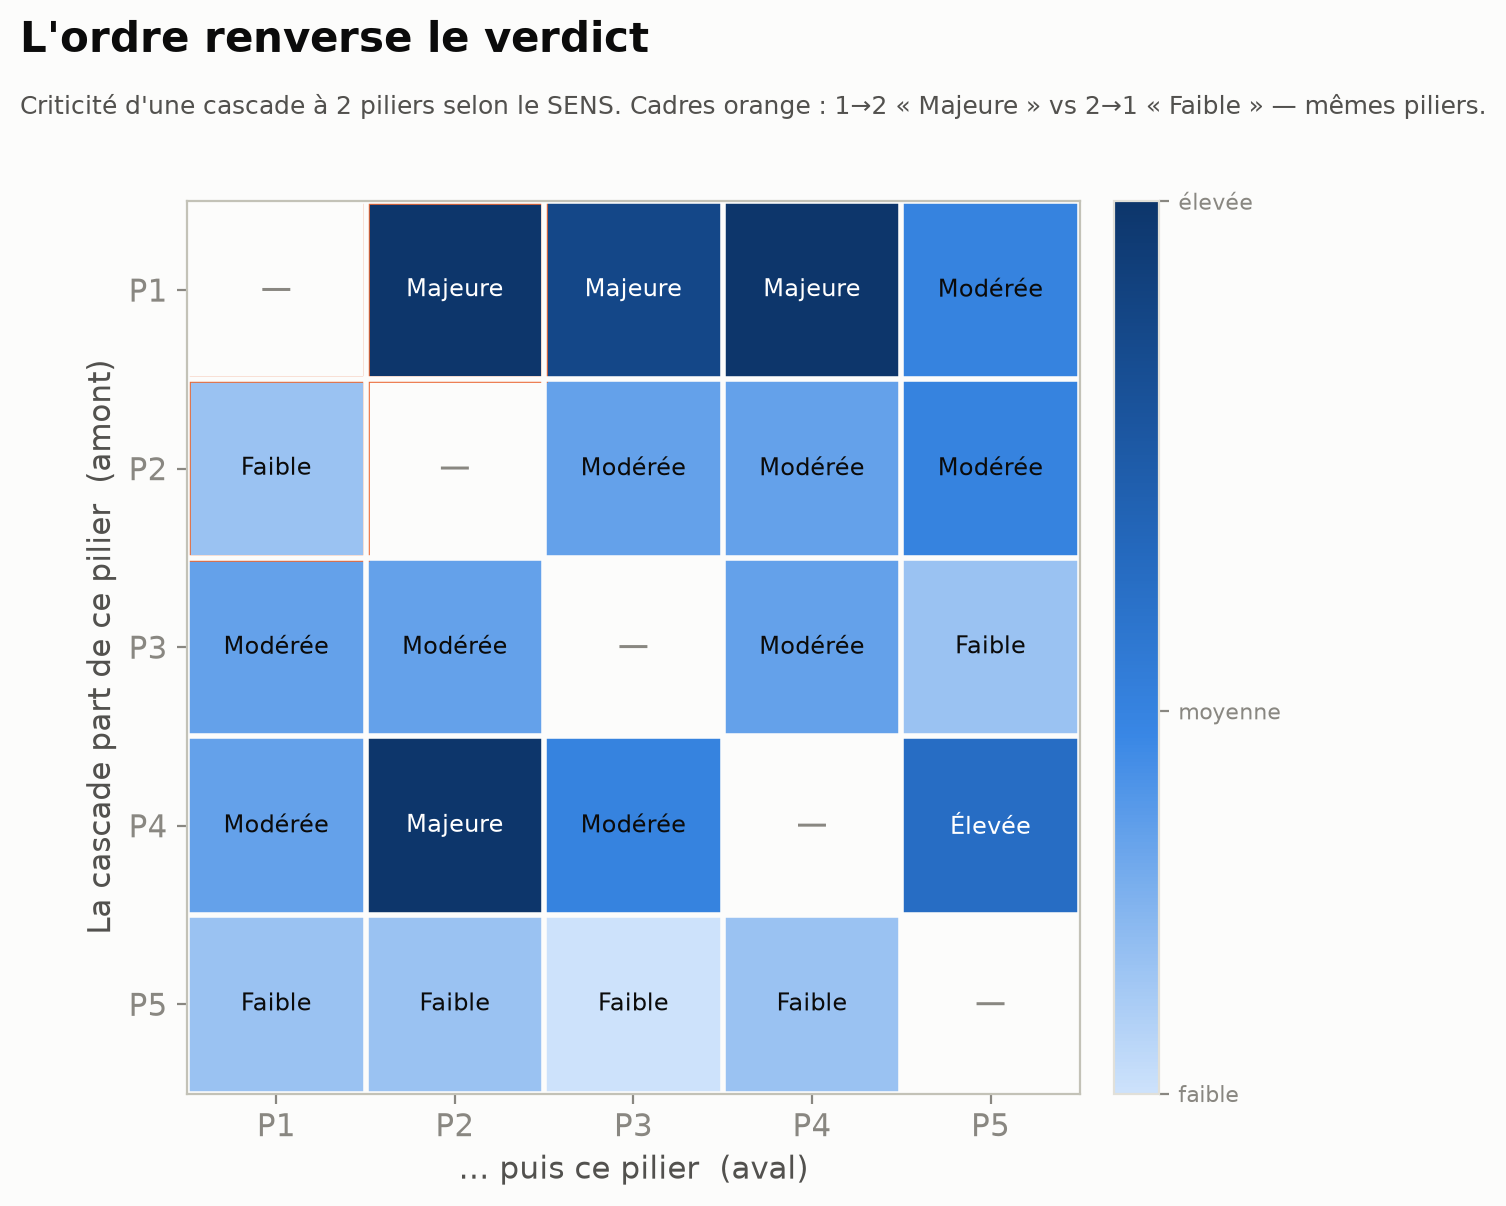
\includegraphics[width=0.78\linewidth]{F1_asymetrie_ordre.png}
\end{center}
\begin{itemize}
\item L'asymétrie de l'ordre est visible sur toutes les paires : ce n'est pas une
      corrélation (une corrélation serait symétrique).
\item Pilier racine dominant : \textbf{P1 gouvernance}, puis P4 tiers
      (classement $P1 > P4 > P2 > P3 > P5$).
\end{itemize}
\end{frame}

% =====================================================================
\begin{frame}{À quoi ça sert : probas conditionnelles au sein d'un même $N_{i,j}$}
$N_{i,j}$ : nombre d'incidents entrant par le pilier $j$ (segment $i$).
La cascade ne touche pas la fréquence, elle vit \textbf{dans la loi conditionnelle} :
\medskip
\begin{itemize}
\item sachant $N_{i,j} = n$, chacun des $n$ incidents part de $j$ et entraîne $j'$ avec
\[
\mathbb{P}(j' \mid j) \;=\; \frac{\texttt{TRANS}(j)(j')}{s_j},
\qquad s_j = \textstyle\sum_{k} \texttt{TRANS}(j)(k) ;
\]
\item l'incident touche donc un \textbf{ensemble} de piliers (pas un seul), et la sévérité
      de la cellule est une somme composée
      $S_{i,j} = \sum_{k=1}^{N_{i,j}} X_k$, chaque $X_k$ gonflé par la cascade.
\end{itemize}
\medskip
Conséquence pratique : les lois de fréquence restent standard (Poisson, binomiale
négative) ; toute la dépendance entre piliers est portée par le mécanisme.
Estimable sur un registre horodaté : $\widehat{\mathbb{P}}(j'|j) = N_{j,j'} / N_{j,\cdot}$.
\end{frame}

% =====================================================================
\begin{frame}{Fait 2 : la refonte du Vasicek, ce qu'on propose}
\textbf{Point de départ.} Vasicek à un facteur : même corrélation pour tous les piliers,
symétrique. Insuffisant pour DORA (la dépendance y est dirigée).
\medskip
\begin{enumerate}
\item \textbf{Généralisation A} : charge systémique $s_j$ propre à chaque pilier.
\item \textbf{Généralisation B} : propagation dirigée, matrice d'influence $W$
      (construite depuis \texttt{TRANS}) : un incident sur $j$ se propage vers $j'$.
\item \textbf{Normalisation de Leontief} : $W$ renormalisée pour que
      $\rho(W) \le g < 1$. La stabilité est \emph{garantie par construction},
      pas supposée.
\item \textbf{Lecture processus de branchement} : $R_0 = \rho(M) < 1$ ; la progéniture
      par pilier retrouve exactement le classement \texttt{ROOT} (contrôle de cohérence).
\end{enumerate}
\medskip
Le seuil de bascule $K_j$ remplace le $\Phi^{-1}(\mathrm{PD})$ du monde crédit.
\end{frame}

% =====================================================================
\begin{frame}{Où ça mène (aperçu, détail au prochain point)}
L'état de conformité DORA (Non conforme / Partiellement / Conforme) pilote la cascade,
d'où un \textbf{SCR par état} en euros (sévérités SAS OpRisk et PRC) :
\medskip
\begin{itemize}
\item surcoût de non-conformité (NC vs C) : médiane $\sim 7{,}4$~Md\euro{} (OpRisk),
      \textbf{100~\% des tirages bootstrap positifs} ;
\item le classement des piliers obtenu en euros \textbf{reproduit le classement
      d'expert} du classeur qualitatif (validation croisée) ;
\item une trajectoire de capital le long de la mise en conformité (chaîne de Markov),
      et un ordre de remédiation optimal $=$ l'ordre \texttt{ROOT}.
\end{itemize}
\medskip
Verdict transversal : le \textbf{classement} est robuste, le \textbf{niveau} ne l'est pas
(queue lourde) ; on pilote au classement.
\end{frame}

% =====================================================================
\begin{frame}{Points bloquants}
\begin{enumerate}
\item \textbf{Calibrer $W$ (la matrice de propagation).} Aucune source publique ne
      permet de l'estimer : OpRisk ne code pas les piliers co-touchés, la PRC n'a pas
      l'horodatage fin. Il faudrait un \textbf{registre d'incidents horodaté} (format
      reporting DORA). En attendant : jugement d'expert $+$ analyses de sensibilité.
\item \textbf{Le canal détection.} Une entité conforme détecte plus tôt (moins
      d'incidents matériels). L'inclure dans le chiffre de tête ou le laisser en
      sensibilité ? \textbf{À trancher ensemble.}
\item \textbf{Le niveau du capital n'est pas pinçable} (indice de queue $\xi$, intervalle
      large). Assumé dans la rédaction : la direction et le classement sont certains,
      le niveau est une distribution.
\end{enumerate}
\end{frame}

% =====================================================================
\begin{frame}{Pour la prochaine fois}
\begin{enumerate}
\item \textbf{Assembler le document complet} : les trois chapitres neufs (cascade,
      multi-états, résultats) sont rédigés ; migrer les parties agnostiques de l'ancien
      mémoire (introduction, état de l'art, données, annexes EVT).
\item \textbf{Trancher le canal détection} (point 2 des bloquants) : les deux lectures
      sont déjà chiffrées, la décision ne bloque pas le reste.
\item \textbf{Figer l'ancrage} des probabilités d'état (NC 35 / PC 35 / C 30, enquêtes) :
      la sensibilité est faite, il reste à valider le choix central.
\item Si accessible : explorer la piste \textbf{registre d'incidents} pour une première
      calibration de $W$.
\end{enumerate}
\end{frame}

\end{document}
